
% Default to the notebook output style

    


% Inherit from the specified cell style.




    
\documentclass{article}

    
    
    \usepackage{graphicx} % Used to insert images
    \usepackage{adjustbox} % Used to constrain images to a maximum size 
    \usepackage{color} % Allow colors to be defined
    \usepackage{enumerate} % Needed for markdown enumerations to work
    \usepackage{geometry} % Used to adjust the document margins
    \usepackage{amsmath} % Equations
    \usepackage{amssymb} % Equations
    \usepackage[mathletters]{ucs} % Extended unicode (utf-8) support
    \usepackage[utf8x]{inputenc} % Allow utf-8 characters in the tex document
    \usepackage{fancyvrb} % verbatim replacement that allows latex
    \usepackage{grffile} % extends the file name processing of package graphics 
                         % to support a larger range 
    % The hyperref package gives us a pdf with properly built
    % internal navigation ('pdf bookmarks' for the table of contents,
    % internal cross-reference links, web links for URLs, etc.)
    \usepackage{hyperref}
    \usepackage{longtable} % longtable support required by pandoc >1.10
    

    
    
    \definecolor{orange}{cmyk}{0,0.4,0.8,0.2}
    \definecolor{darkorange}{rgb}{.71,0.21,0.01}
    \definecolor{darkgreen}{rgb}{.12,.54,.11}
    \definecolor{myteal}{rgb}{.26, .44, .56}
    \definecolor{gray}{gray}{0.45}
    \definecolor{lightgray}{gray}{.95}
    \definecolor{mediumgray}{gray}{.8}
    \definecolor{inputbackground}{rgb}{.95, .95, .85}
    \definecolor{outputbackground}{rgb}{.95, .95, .95}
    \definecolor{traceback}{rgb}{1, .95, .95}
    % ansi colors
    \definecolor{red}{rgb}{.6,0,0}
    \definecolor{green}{rgb}{0,.65,0}
    \definecolor{brown}{rgb}{0.6,0.6,0}
    \definecolor{blue}{rgb}{0,.145,.698}
    \definecolor{purple}{rgb}{.698,.145,.698}
    \definecolor{cyan}{rgb}{0,.698,.698}
    \definecolor{lightgray}{gray}{0.5}
    
    % bright ansi colors
    \definecolor{darkgray}{gray}{0.25}
    \definecolor{lightred}{rgb}{1.0,0.39,0.28}
    \definecolor{lightgreen}{rgb}{0.48,0.99,0.0}
    \definecolor{lightblue}{rgb}{0.53,0.81,0.92}
    \definecolor{lightpurple}{rgb}{0.87,0.63,0.87}
    \definecolor{lightcyan}{rgb}{0.5,1.0,0.83}
    
    % commands and environments needed by pandoc snippets
    % extracted from the output of `pandoc -s`
    \DefineVerbatimEnvironment{Highlighting}{Verbatim}{commandchars=\\\{\}}
    % Add ',fontsize=\small' for more characters per line
    \newenvironment{Shaded}{}{}
    \newcommand{\KeywordTok}[1]{\textcolor[rgb]{0.00,0.44,0.13}{\textbf{{#1}}}}
    \newcommand{\DataTypeTok}[1]{\textcolor[rgb]{0.56,0.13,0.00}{{#1}}}
    \newcommand{\DecValTok}[1]{\textcolor[rgb]{0.25,0.63,0.44}{{#1}}}
    \newcommand{\BaseNTok}[1]{\textcolor[rgb]{0.25,0.63,0.44}{{#1}}}
    \newcommand{\FloatTok}[1]{\textcolor[rgb]{0.25,0.63,0.44}{{#1}}}
    \newcommand{\CharTok}[1]{\textcolor[rgb]{0.25,0.44,0.63}{{#1}}}
    \newcommand{\StringTok}[1]{\textcolor[rgb]{0.25,0.44,0.63}{{#1}}}
    \newcommand{\CommentTok}[1]{\textcolor[rgb]{0.38,0.63,0.69}{\textit{{#1}}}}
    \newcommand{\OtherTok}[1]{\textcolor[rgb]{0.00,0.44,0.13}{{#1}}}
    \newcommand{\AlertTok}[1]{\textcolor[rgb]{1.00,0.00,0.00}{\textbf{{#1}}}}
    \newcommand{\FunctionTok}[1]{\textcolor[rgb]{0.02,0.16,0.49}{{#1}}}
    \newcommand{\RegionMarkerTok}[1]{{#1}}
    \newcommand{\ErrorTok}[1]{\textcolor[rgb]{1.00,0.00,0.00}{\textbf{{#1}}}}
    \newcommand{\NormalTok}[1]{{#1}}
    
    % Define a nice break command that doesn't care if a line doesn't already
    % exist.
    \def\br{\hspace*{\fill} \\* }
    % Math Jax compatability definitions
    \def\gt{>}
    \def\lt{<}
    % Document parameters
    \title{lamprey\_rnaseq\_sample\_comp}
    
    
    

    % Pygments definitions
    
\makeatletter
\def\PY@reset{\let\PY@it=\relax \let\PY@bf=\relax%
    \let\PY@ul=\relax \let\PY@tc=\relax%
    \let\PY@bc=\relax \let\PY@ff=\relax}
\def\PY@tok#1{\csname PY@tok@#1\endcsname}
\def\PY@toks#1+{\ifx\relax#1\empty\else%
    \PY@tok{#1}\expandafter\PY@toks\fi}
\def\PY@do#1{\PY@bc{\PY@tc{\PY@ul{%
    \PY@it{\PY@bf{\PY@ff{#1}}}}}}}
\def\PY#1#2{\PY@reset\PY@toks#1+\relax+\PY@do{#2}}

\expandafter\def\csname PY@tok@gd\endcsname{\def\PY@tc##1{\textcolor[rgb]{0.63,0.00,0.00}{##1}}}
\expandafter\def\csname PY@tok@gu\endcsname{\let\PY@bf=\textbf\def\PY@tc##1{\textcolor[rgb]{0.50,0.00,0.50}{##1}}}
\expandafter\def\csname PY@tok@gt\endcsname{\def\PY@tc##1{\textcolor[rgb]{0.00,0.27,0.87}{##1}}}
\expandafter\def\csname PY@tok@gs\endcsname{\let\PY@bf=\textbf}
\expandafter\def\csname PY@tok@gr\endcsname{\def\PY@tc##1{\textcolor[rgb]{1.00,0.00,0.00}{##1}}}
\expandafter\def\csname PY@tok@cm\endcsname{\let\PY@it=\textit\def\PY@tc##1{\textcolor[rgb]{0.25,0.50,0.50}{##1}}}
\expandafter\def\csname PY@tok@vg\endcsname{\def\PY@tc##1{\textcolor[rgb]{0.10,0.09,0.49}{##1}}}
\expandafter\def\csname PY@tok@m\endcsname{\def\PY@tc##1{\textcolor[rgb]{0.40,0.40,0.40}{##1}}}
\expandafter\def\csname PY@tok@mh\endcsname{\def\PY@tc##1{\textcolor[rgb]{0.40,0.40,0.40}{##1}}}
\expandafter\def\csname PY@tok@go\endcsname{\def\PY@tc##1{\textcolor[rgb]{0.53,0.53,0.53}{##1}}}
\expandafter\def\csname PY@tok@ge\endcsname{\let\PY@it=\textit}
\expandafter\def\csname PY@tok@vc\endcsname{\def\PY@tc##1{\textcolor[rgb]{0.10,0.09,0.49}{##1}}}
\expandafter\def\csname PY@tok@il\endcsname{\def\PY@tc##1{\textcolor[rgb]{0.40,0.40,0.40}{##1}}}
\expandafter\def\csname PY@tok@cs\endcsname{\let\PY@it=\textit\def\PY@tc##1{\textcolor[rgb]{0.25,0.50,0.50}{##1}}}
\expandafter\def\csname PY@tok@cp\endcsname{\def\PY@tc##1{\textcolor[rgb]{0.74,0.48,0.00}{##1}}}
\expandafter\def\csname PY@tok@gi\endcsname{\def\PY@tc##1{\textcolor[rgb]{0.00,0.63,0.00}{##1}}}
\expandafter\def\csname PY@tok@gh\endcsname{\let\PY@bf=\textbf\def\PY@tc##1{\textcolor[rgb]{0.00,0.00,0.50}{##1}}}
\expandafter\def\csname PY@tok@ni\endcsname{\let\PY@bf=\textbf\def\PY@tc##1{\textcolor[rgb]{0.60,0.60,0.60}{##1}}}
\expandafter\def\csname PY@tok@nl\endcsname{\def\PY@tc##1{\textcolor[rgb]{0.63,0.63,0.00}{##1}}}
\expandafter\def\csname PY@tok@nn\endcsname{\let\PY@bf=\textbf\def\PY@tc##1{\textcolor[rgb]{0.00,0.00,1.00}{##1}}}
\expandafter\def\csname PY@tok@no\endcsname{\def\PY@tc##1{\textcolor[rgb]{0.53,0.00,0.00}{##1}}}
\expandafter\def\csname PY@tok@na\endcsname{\def\PY@tc##1{\textcolor[rgb]{0.49,0.56,0.16}{##1}}}
\expandafter\def\csname PY@tok@nb\endcsname{\def\PY@tc##1{\textcolor[rgb]{0.00,0.50,0.00}{##1}}}
\expandafter\def\csname PY@tok@nc\endcsname{\let\PY@bf=\textbf\def\PY@tc##1{\textcolor[rgb]{0.00,0.00,1.00}{##1}}}
\expandafter\def\csname PY@tok@nd\endcsname{\def\PY@tc##1{\textcolor[rgb]{0.67,0.13,1.00}{##1}}}
\expandafter\def\csname PY@tok@ne\endcsname{\let\PY@bf=\textbf\def\PY@tc##1{\textcolor[rgb]{0.82,0.25,0.23}{##1}}}
\expandafter\def\csname PY@tok@nf\endcsname{\def\PY@tc##1{\textcolor[rgb]{0.00,0.00,1.00}{##1}}}
\expandafter\def\csname PY@tok@si\endcsname{\let\PY@bf=\textbf\def\PY@tc##1{\textcolor[rgb]{0.73,0.40,0.53}{##1}}}
\expandafter\def\csname PY@tok@s2\endcsname{\def\PY@tc##1{\textcolor[rgb]{0.73,0.13,0.13}{##1}}}
\expandafter\def\csname PY@tok@vi\endcsname{\def\PY@tc##1{\textcolor[rgb]{0.10,0.09,0.49}{##1}}}
\expandafter\def\csname PY@tok@nt\endcsname{\let\PY@bf=\textbf\def\PY@tc##1{\textcolor[rgb]{0.00,0.50,0.00}{##1}}}
\expandafter\def\csname PY@tok@nv\endcsname{\def\PY@tc##1{\textcolor[rgb]{0.10,0.09,0.49}{##1}}}
\expandafter\def\csname PY@tok@s1\endcsname{\def\PY@tc##1{\textcolor[rgb]{0.73,0.13,0.13}{##1}}}
\expandafter\def\csname PY@tok@sh\endcsname{\def\PY@tc##1{\textcolor[rgb]{0.73,0.13,0.13}{##1}}}
\expandafter\def\csname PY@tok@sc\endcsname{\def\PY@tc##1{\textcolor[rgb]{0.73,0.13,0.13}{##1}}}
\expandafter\def\csname PY@tok@sx\endcsname{\def\PY@tc##1{\textcolor[rgb]{0.00,0.50,0.00}{##1}}}
\expandafter\def\csname PY@tok@bp\endcsname{\def\PY@tc##1{\textcolor[rgb]{0.00,0.50,0.00}{##1}}}
\expandafter\def\csname PY@tok@c1\endcsname{\let\PY@it=\textit\def\PY@tc##1{\textcolor[rgb]{0.25,0.50,0.50}{##1}}}
\expandafter\def\csname PY@tok@kc\endcsname{\let\PY@bf=\textbf\def\PY@tc##1{\textcolor[rgb]{0.00,0.50,0.00}{##1}}}
\expandafter\def\csname PY@tok@c\endcsname{\let\PY@it=\textit\def\PY@tc##1{\textcolor[rgb]{0.25,0.50,0.50}{##1}}}
\expandafter\def\csname PY@tok@mf\endcsname{\def\PY@tc##1{\textcolor[rgb]{0.40,0.40,0.40}{##1}}}
\expandafter\def\csname PY@tok@err\endcsname{\def\PY@bc##1{\setlength{\fboxsep}{0pt}\fcolorbox[rgb]{1.00,0.00,0.00}{1,1,1}{\strut ##1}}}
\expandafter\def\csname PY@tok@kd\endcsname{\let\PY@bf=\textbf\def\PY@tc##1{\textcolor[rgb]{0.00,0.50,0.00}{##1}}}
\expandafter\def\csname PY@tok@ss\endcsname{\def\PY@tc##1{\textcolor[rgb]{0.10,0.09,0.49}{##1}}}
\expandafter\def\csname PY@tok@sr\endcsname{\def\PY@tc##1{\textcolor[rgb]{0.73,0.40,0.53}{##1}}}
\expandafter\def\csname PY@tok@mo\endcsname{\def\PY@tc##1{\textcolor[rgb]{0.40,0.40,0.40}{##1}}}
\expandafter\def\csname PY@tok@kn\endcsname{\let\PY@bf=\textbf\def\PY@tc##1{\textcolor[rgb]{0.00,0.50,0.00}{##1}}}
\expandafter\def\csname PY@tok@mi\endcsname{\def\PY@tc##1{\textcolor[rgb]{0.40,0.40,0.40}{##1}}}
\expandafter\def\csname PY@tok@gp\endcsname{\let\PY@bf=\textbf\def\PY@tc##1{\textcolor[rgb]{0.00,0.00,0.50}{##1}}}
\expandafter\def\csname PY@tok@o\endcsname{\def\PY@tc##1{\textcolor[rgb]{0.40,0.40,0.40}{##1}}}
\expandafter\def\csname PY@tok@kr\endcsname{\let\PY@bf=\textbf\def\PY@tc##1{\textcolor[rgb]{0.00,0.50,0.00}{##1}}}
\expandafter\def\csname PY@tok@s\endcsname{\def\PY@tc##1{\textcolor[rgb]{0.73,0.13,0.13}{##1}}}
\expandafter\def\csname PY@tok@kp\endcsname{\def\PY@tc##1{\textcolor[rgb]{0.00,0.50,0.00}{##1}}}
\expandafter\def\csname PY@tok@w\endcsname{\def\PY@tc##1{\textcolor[rgb]{0.73,0.73,0.73}{##1}}}
\expandafter\def\csname PY@tok@kt\endcsname{\def\PY@tc##1{\textcolor[rgb]{0.69,0.00,0.25}{##1}}}
\expandafter\def\csname PY@tok@ow\endcsname{\let\PY@bf=\textbf\def\PY@tc##1{\textcolor[rgb]{0.67,0.13,1.00}{##1}}}
\expandafter\def\csname PY@tok@sb\endcsname{\def\PY@tc##1{\textcolor[rgb]{0.73,0.13,0.13}{##1}}}
\expandafter\def\csname PY@tok@k\endcsname{\let\PY@bf=\textbf\def\PY@tc##1{\textcolor[rgb]{0.00,0.50,0.00}{##1}}}
\expandafter\def\csname PY@tok@se\endcsname{\let\PY@bf=\textbf\def\PY@tc##1{\textcolor[rgb]{0.73,0.40,0.13}{##1}}}
\expandafter\def\csname PY@tok@sd\endcsname{\let\PY@it=\textit\def\PY@tc##1{\textcolor[rgb]{0.73,0.13,0.13}{##1}}}

\def\PYZbs{\char`\\}
\def\PYZus{\char`\_}
\def\PYZob{\char`\{}
\def\PYZcb{\char`\}}
\def\PYZca{\char`\^}
\def\PYZam{\char`\&}
\def\PYZlt{\char`\<}
\def\PYZgt{\char`\>}
\def\PYZsh{\char`\#}
\def\PYZpc{\char`\%}
\def\PYZdl{\char`\$}
\def\PYZhy{\char`\-}
\def\PYZsq{\char`\'}
\def\PYZdq{\char`\"}
\def\PYZti{\char`\~}
% for compatibility with earlier versions
\def\PYZat{@}
\def\PYZlb{[}
\def\PYZrb{]}
\makeatother


    % Exact colors from NB
    \definecolor{incolor}{rgb}{0.0, 0.0, 0.5}
    \definecolor{outcolor}{rgb}{0.545, 0.0, 0.0}



    
    % Prevent overflowing lines due to hard-to-break entities
    \sloppy 
    % Setup hyperref package
    \hypersetup{
      breaklinks=true,  % so long urls are correctly broken across lines
      colorlinks=true,
      urlcolor=blue,
      linkcolor=darkorange,
      citecolor=darkgreen,
      }
    % Slightly bigger margins than the latex defaults
    
    \geometry{verbose,tmargin=1in,bmargin=1in,lmargin=1in,rmargin=1in}
    
    

    \begin{document}
    
    
    \maketitle
    
    

    

    \section{Lamprey RNA-Seq 2014}



    \subsection{Between-sample Assembly Comparison}



    \subsubsection{Camille Scott (camille.scott.w@gmail.com) Michigan State University GED
Lab}



    \subsubsection{https://github.com/camillescott/2013-lamprey/tree/lamp3}



    \subsection{Overview}


    The primary goal of this project has been to produce a scientifically
usable set of transcripts from our vast collection of RNA-seq samples.
Given the lack of completeness of the current lamprey genome, we chose
to assemble the reads de novo, using our in-house pipeline. The basics
of the assembly pipeline can be found in the
\emph{\href{https://khmer-protocols.readthedocs.org/en/v0.8.4/mrnaseq/}{Eel
Pond protocol}}.

This document goes over the content of the resulting assembly with
respect to each sample used to construct it. We align every sample to
the assembly, and use an abundance estimation tool to get expression
levels for each transcript, for each sample. This allows us to analyze
the extent to which each sample contributed to the final assembly, and
the relative representation of each sample within the assembly. We
consider a transcript \emph{represented} in a sample if it has an
estimated abundance greater than 1.0 from the reads in that sample.

An overview of the samples can be found
\href{https://docs.google.com/spreadsheet/ccc?key=0AqkPW_VPT5rAdEdmczhDeWg4UEZWdmh4dElqeXFiUlE\&usp=sharing}{here}.
This is what I have been able to scrape up from various collaborators
and sequencing centers; some information is definitely missing, and some
samples were preprocessed before being given to me. As such, any
comments on this document are greatly appreciated, whether they be
corrections or offers for original versions of the data. Note that the
second sheet has the key between the original sample names and the id's
being used in the current project.

For all plots, ``filtered'' means after the removal of known
contaminants.

All the plots shown in this notebook, as well as many more supporting
figures, can be found in the full notebook in the previously linked
github repository, and can be viewed in rendered form
\emph{\href{http://nbviewer.ipython.org/github/camillescott/2013-lamprey/blob/lamp3/pub/tale_of_two_transcriptomes_compute.ipynb}{here}}.


    \subsection{Validation}


    Briefly, we can show that the assembly is both valid and contains new
information with homologies to model organisms. Here, we show:

\begin{enumerate}
\def\labelenumi{\arabic{enumi}.}
\item
  \emph{\textbf{Putative new:}} Transcripts with substantial protein
  homology to a model species (mouse, zebrafish, or amphioxus) or
  substantial nucleotide homology to the lamprey genome, but no homology
  with the existing lamprey transcripts or ESTs.
\item
  \emph{\textbf{All pututive:}} Transcripts which have homologies in any
  one of the model species, the lamprey genome, lamprey transcripts, or
  lamprey ESTs.
\end{enumerate}

This is done for the transcripts represented in each sample:

\begin{figure}[htbp]
\centering
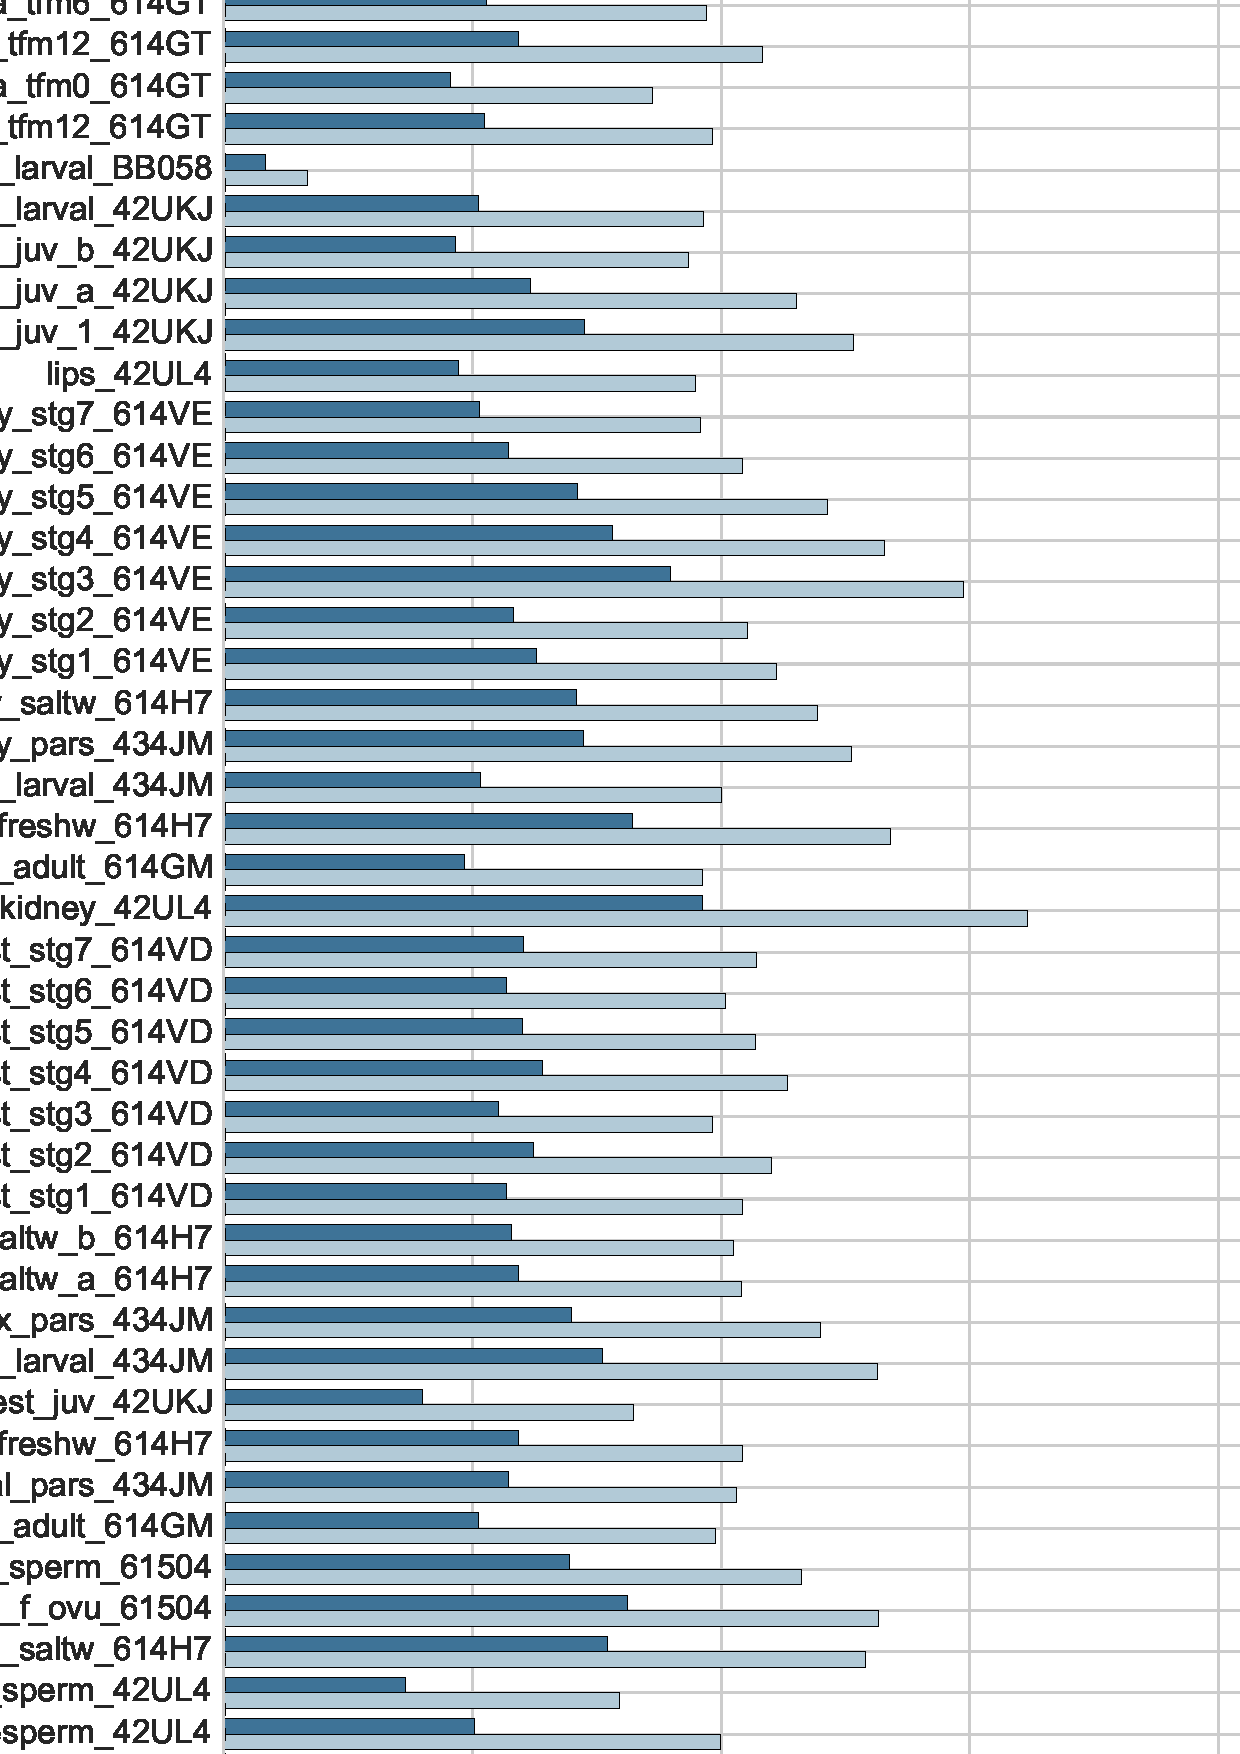
\includegraphics{filtered_putative_transcripts.svg}
\caption{filtered\_putative\_transcripts}
\end{figure}

Note that there is overlap between bars; that is, the sum under the
``curve'' is much greater than the total number of transcripts in the
assembly.

With that in mind, the distribution of the number of samples in which a
transcript is represented, along with genome homologies for each bin:

\begin{figure}[htbp]
\centering
\includegraphics{transcript_sample_dist_support.svg}
\caption{transcript\_sample\_dist\_support}
\end{figure}


    \subsection{Sample Comparison}


    Between sample comparisons seek to analyze both the transcript content
and transcript expression of different samples. The manner in which
these metrics is analyzed depends mostly on the \emph{distance} metric
used.

Briefly, let us have an assembly $T$, consisting of transcripts
$T=\{t_0,t_1,...,t_n\}$, where there are $n$ transcripts total. Let us
also have a set of samples $S$, were $S=\{s_0,s_1,...,s_m\}$, with $m$
samples total; In our case, $m=84$.

Then each sample $s_i$ is a vector
$\bar{s_i}=[ A_i(t_0),A_i(t_1),...,A_i(t_n) ]^T $, where

\[A_i(t_j) = \begin{cases}
1, & \text{if estimated abundance of transcript } t_j \text{ in sample } i \text{ is } > 1.0 \\
0, & \text{otherwise}
\end{cases}\]

for simple sample transcript content, and

\[A_i(t_j) = \text{estimated abundance of transcript } t_j \text{ in sample } i\]

for sample expression.

We then need only define a distance metric $D(s_a,s_b)$ two compare two
samples. This facilitates clustering and tree-building between all pairs
of samples.

\emph{\textbf{In qualitative terms}}, we simply have 84 lists, 1 for
each sample, each of which is a list of estimated abundances for each
transcript. We'll do pairwise comparisons of these lists.

The other important important choice is the clustering method. Two
methods will be demonstrated: the \emph{centroid} method and the
\emph{ward} method. There are decent descriptions of these in the
\href{http://docs.scipy.org/doc/scipy-0.13.0/reference/generated/scipy.cluster.hierarchy.linkage.html}{scipy
clustering docs}, with more detailed descriptions on wikipedia and in
many textbooks and papers. Briefly, in the \emph{centroid} method, the
distance between two clusters is the distance between the mean positions
of all elements in the clusters. It is noted as being robusts to
outliers, but potentially performing worse than other methods. In the
\emph{Ward} method, the distance between two clusters is the
\emph{ANOVA} sum of squares between the two clusters; we seek to
minimize the within-cluster sum of squares distance. \emph{Ward}'s
method performs well with small $N$, and is strongly biased toward
producing clusters with the same number of observations. See
\href{http://v8doc.sas.com/sashtml/stat/chap23/sect12.htm}{here} for
these overviews.


    \subsubsection{Sample Content: \emph{Hamming Distance}}


    Hamming distance measures the number of disagreeing positions in a
binary vector, normalized by the length of the vector (number of
transcripts in this case). See the
\href{http://docs.scipy.org/doc/scipy-0.13.0/reference/generated/scipy.spatial.distance.hamming.html\#scipy.spatial.distance.hamming}{scipy
docs} for a detailed description of the metric used in these figures.

Qualitatively, this is a measure of how many transcripts are shared
between the two samples.

\begin{figure}[htbp]
\centering
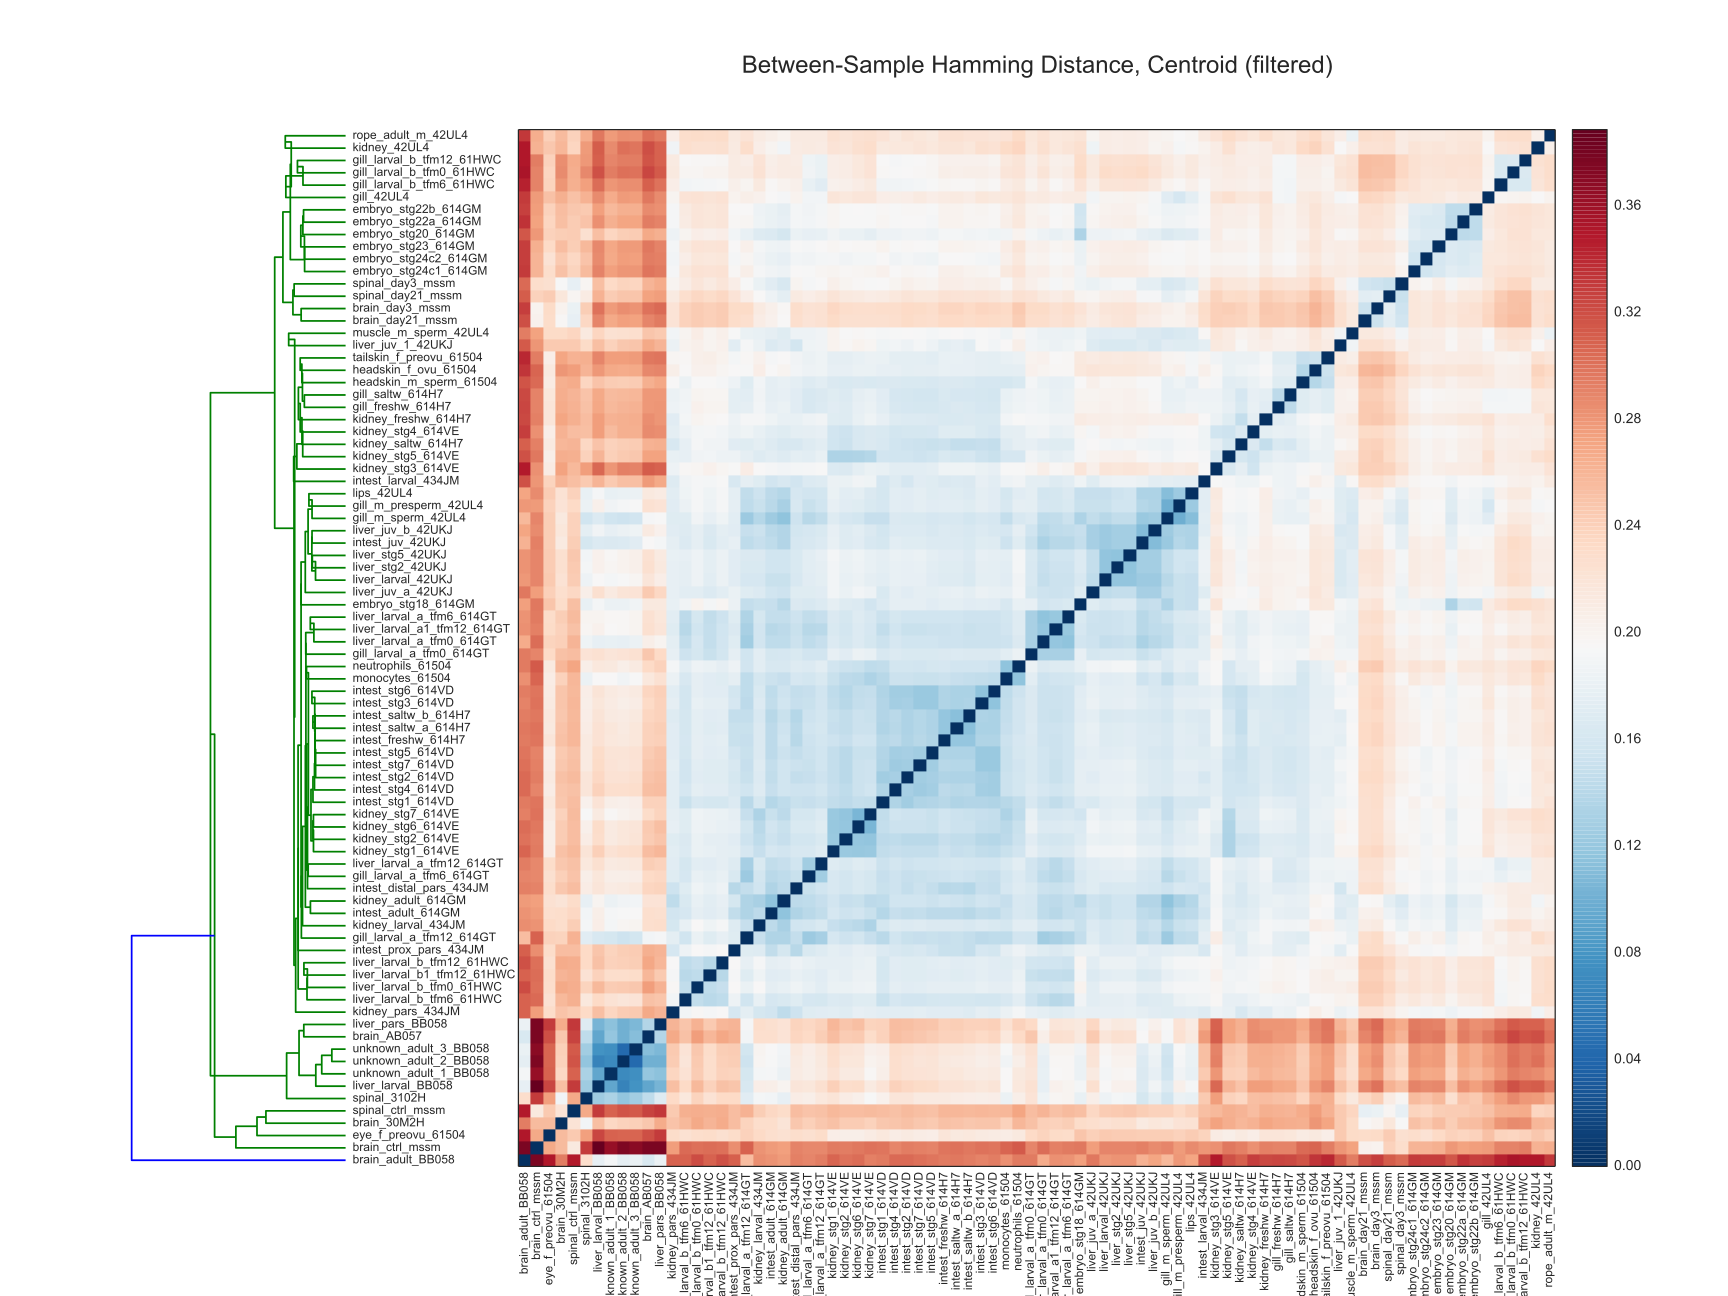
\includegraphics{sample_dendro_hamming_centroid_filtered.svg}
\caption{sample\_dendro\_hamming\_centroid\_filtered}
\end{figure}

\begin{figure}[htbp]
\centering
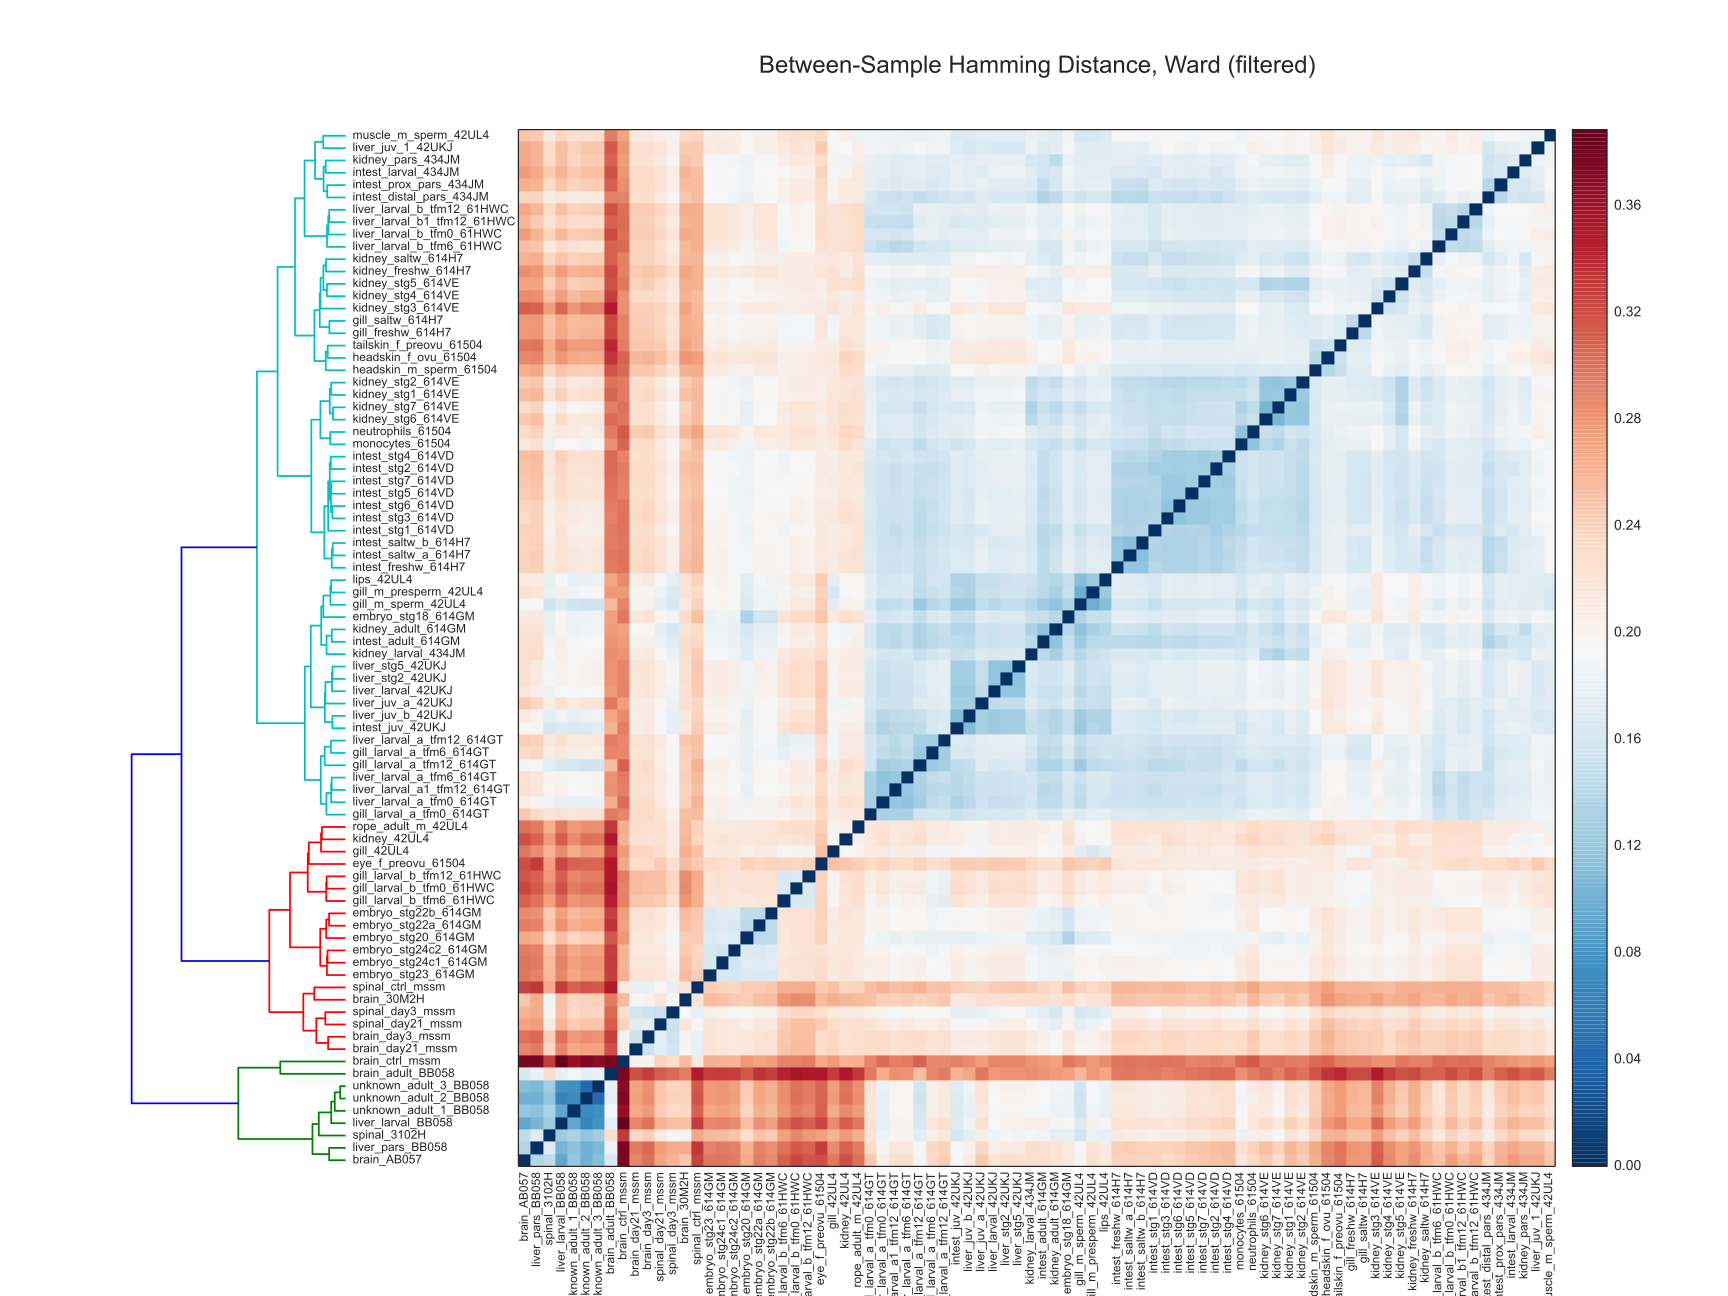
\includegraphics{sample_dendro_hamming_ward_filtered.svg}
\caption{sample\_dendro\_hamming\_ward\_filtered}
\end{figure}

Here, the \emph{Ward} method appears to give better results.


    \subsubsection{Sample Expression: \emph{Correlation Distance}}


    Correlation distance is a measure of the statistical independence of two
distributions. Thus, it will take into account the estimated abundances,
rather than just considering if the transcripts are represented at all,
as in the Hamming distance. The
\href{http://docs.scipy.org/doc/scipy-0.13.0/reference/generated/scipy.spatial.distance.correlation.html\#scipy.spatial.distance.correlation}{scipy
docs} once more have a good description of what was used for this
figure; further information is available on
\href{http://en.wikipedia.org/wiki/Distance_correlation}{wikipedia}.
Notably, while classically a correlation distance of $0.0$ implies
complete statistical independence, this implementation reports
$1-CD(s_a,s_b)$; ie, $1.0$ implies complete statistical independence.

Qualitatively, this is a measure of how similar the distribution of
expression levels (estimated abundances) is between two samples.

\begin{figure}[htbp]
\centering
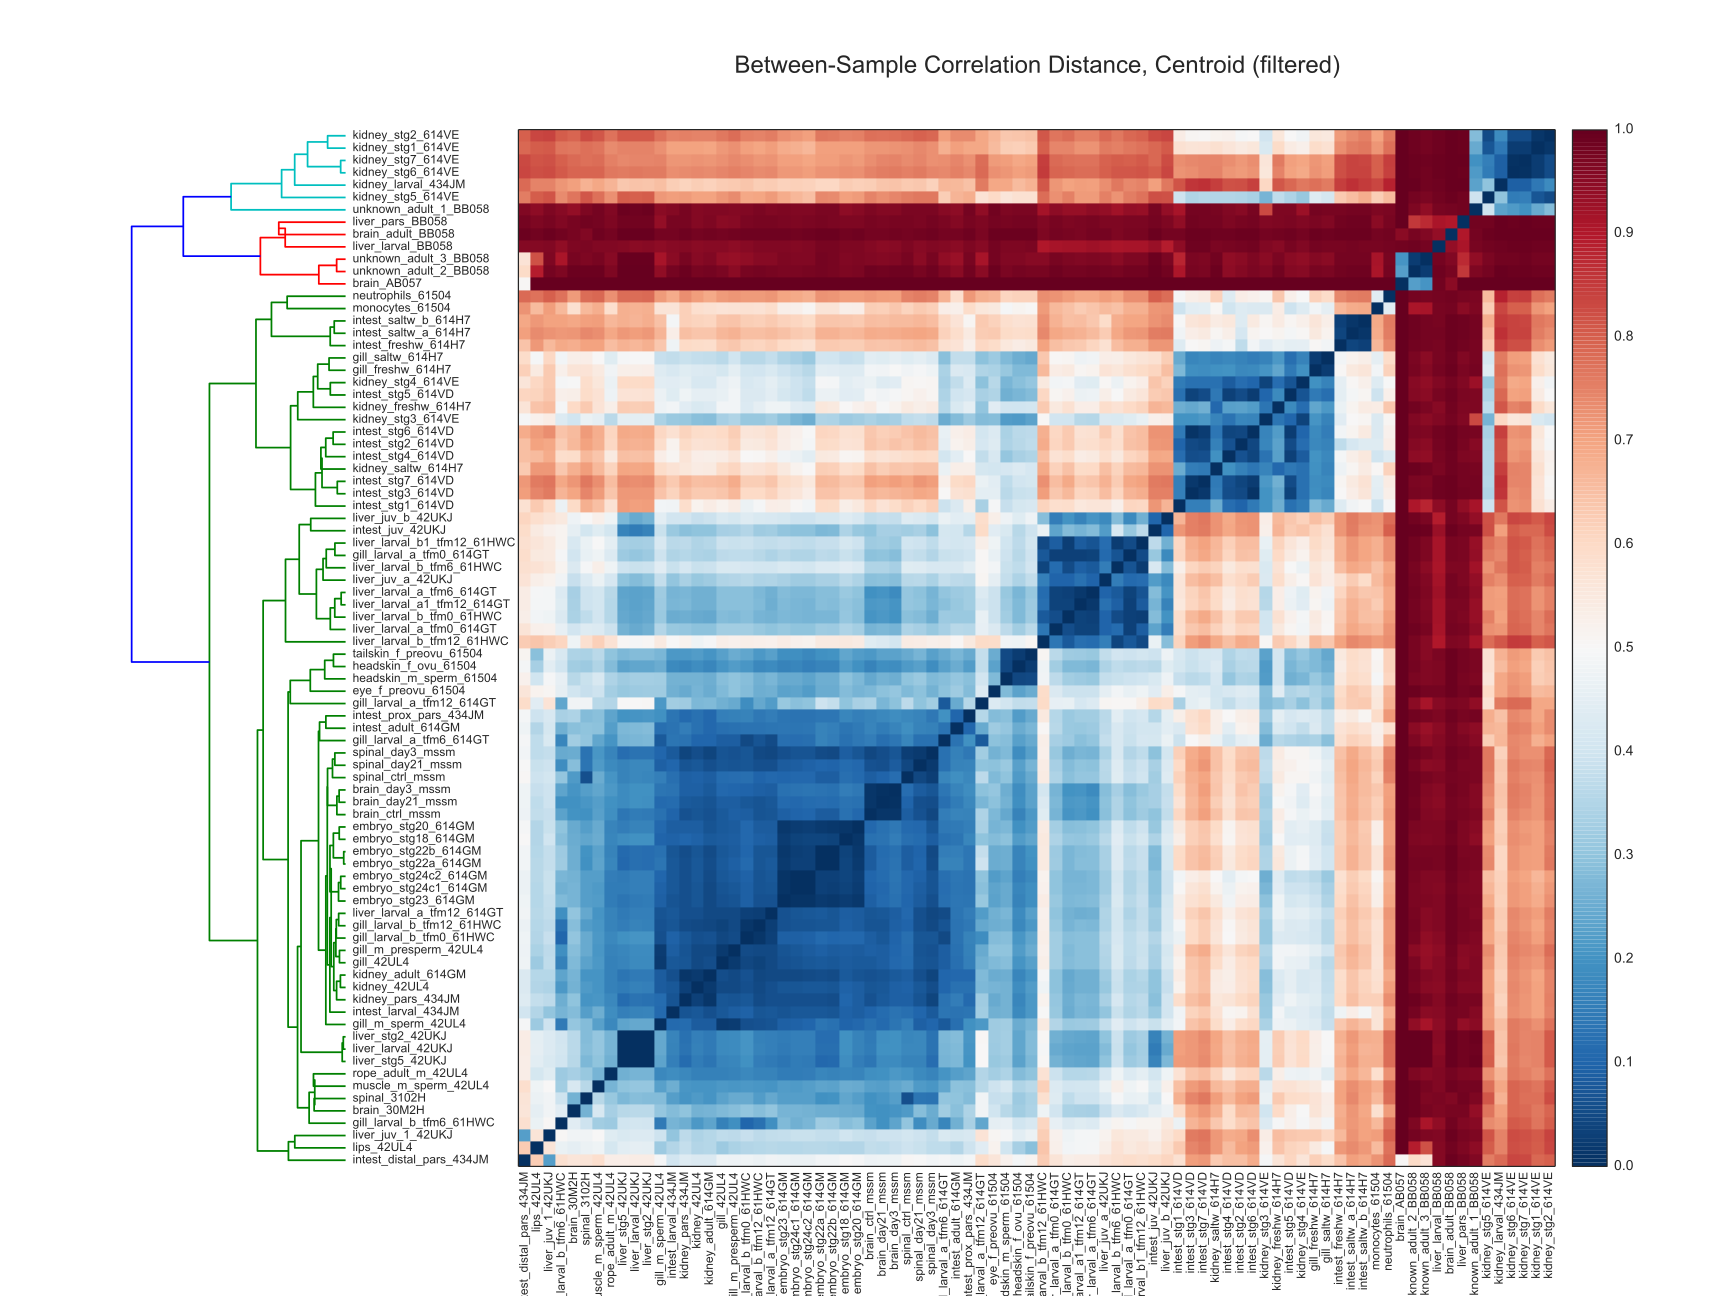
\includegraphics{sample_dendro_correlation_centroid_filtered.svg}
\caption{sample\_dendro\_correlation\_centroid\_filtered}
\end{figure}

\begin{figure}[htbp]
\centering
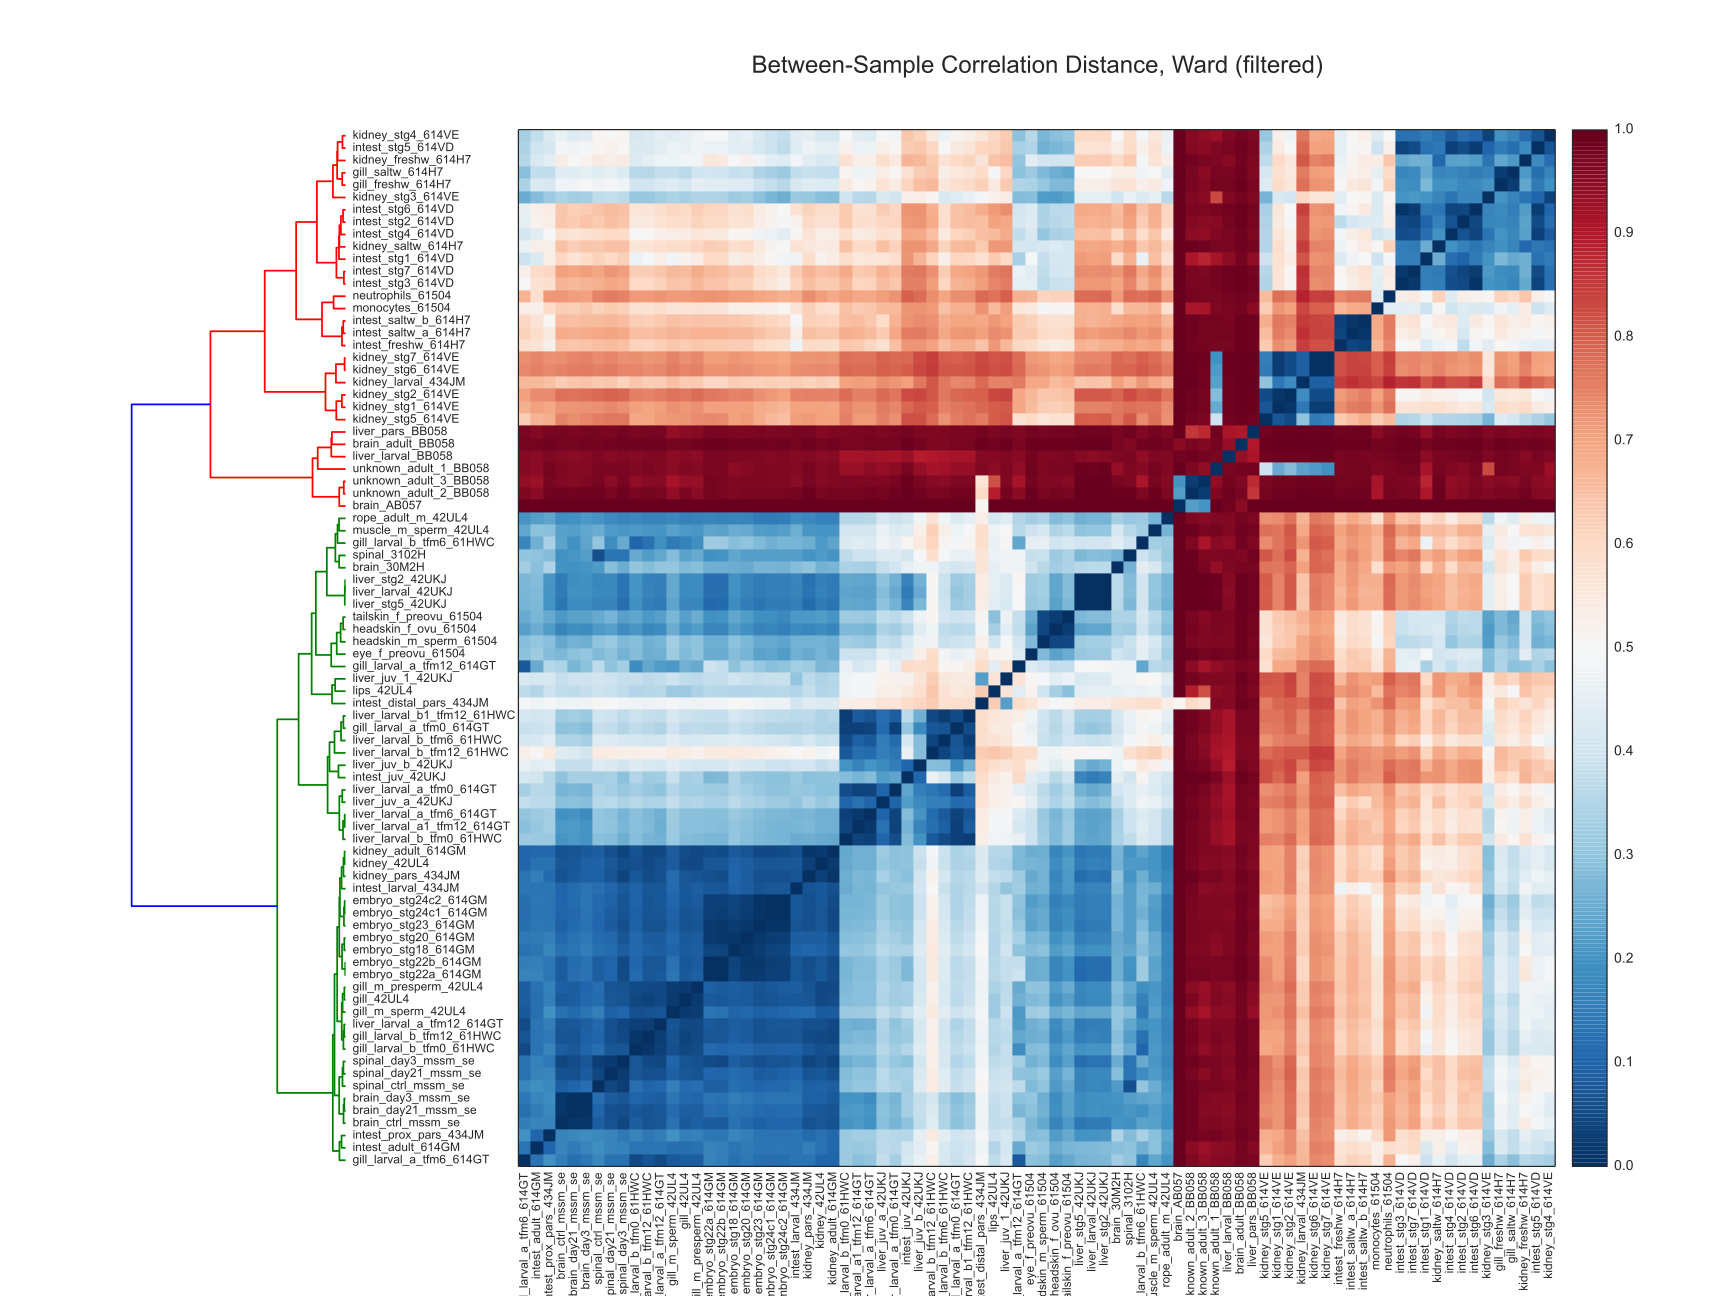
\includegraphics{sample_dendro_correlation_ward_filtered.svg}
\caption{sample\_dendro\_correlation\_ward\_filtered}
\end{figure}


    \subsubsection{Sample Expression: Specific Cases}


    We can also look at how the clustering changes with differing subsets of
transcripts. This could be of interest in regards to evolutionary
changes.

First, we will take transcripts homologous to an amphioxus protein, but
not to mouse or zebrafish. Note that amphioxus shares a common ancestor
with lamprey.

\begin{figure}[htbp]
\centering
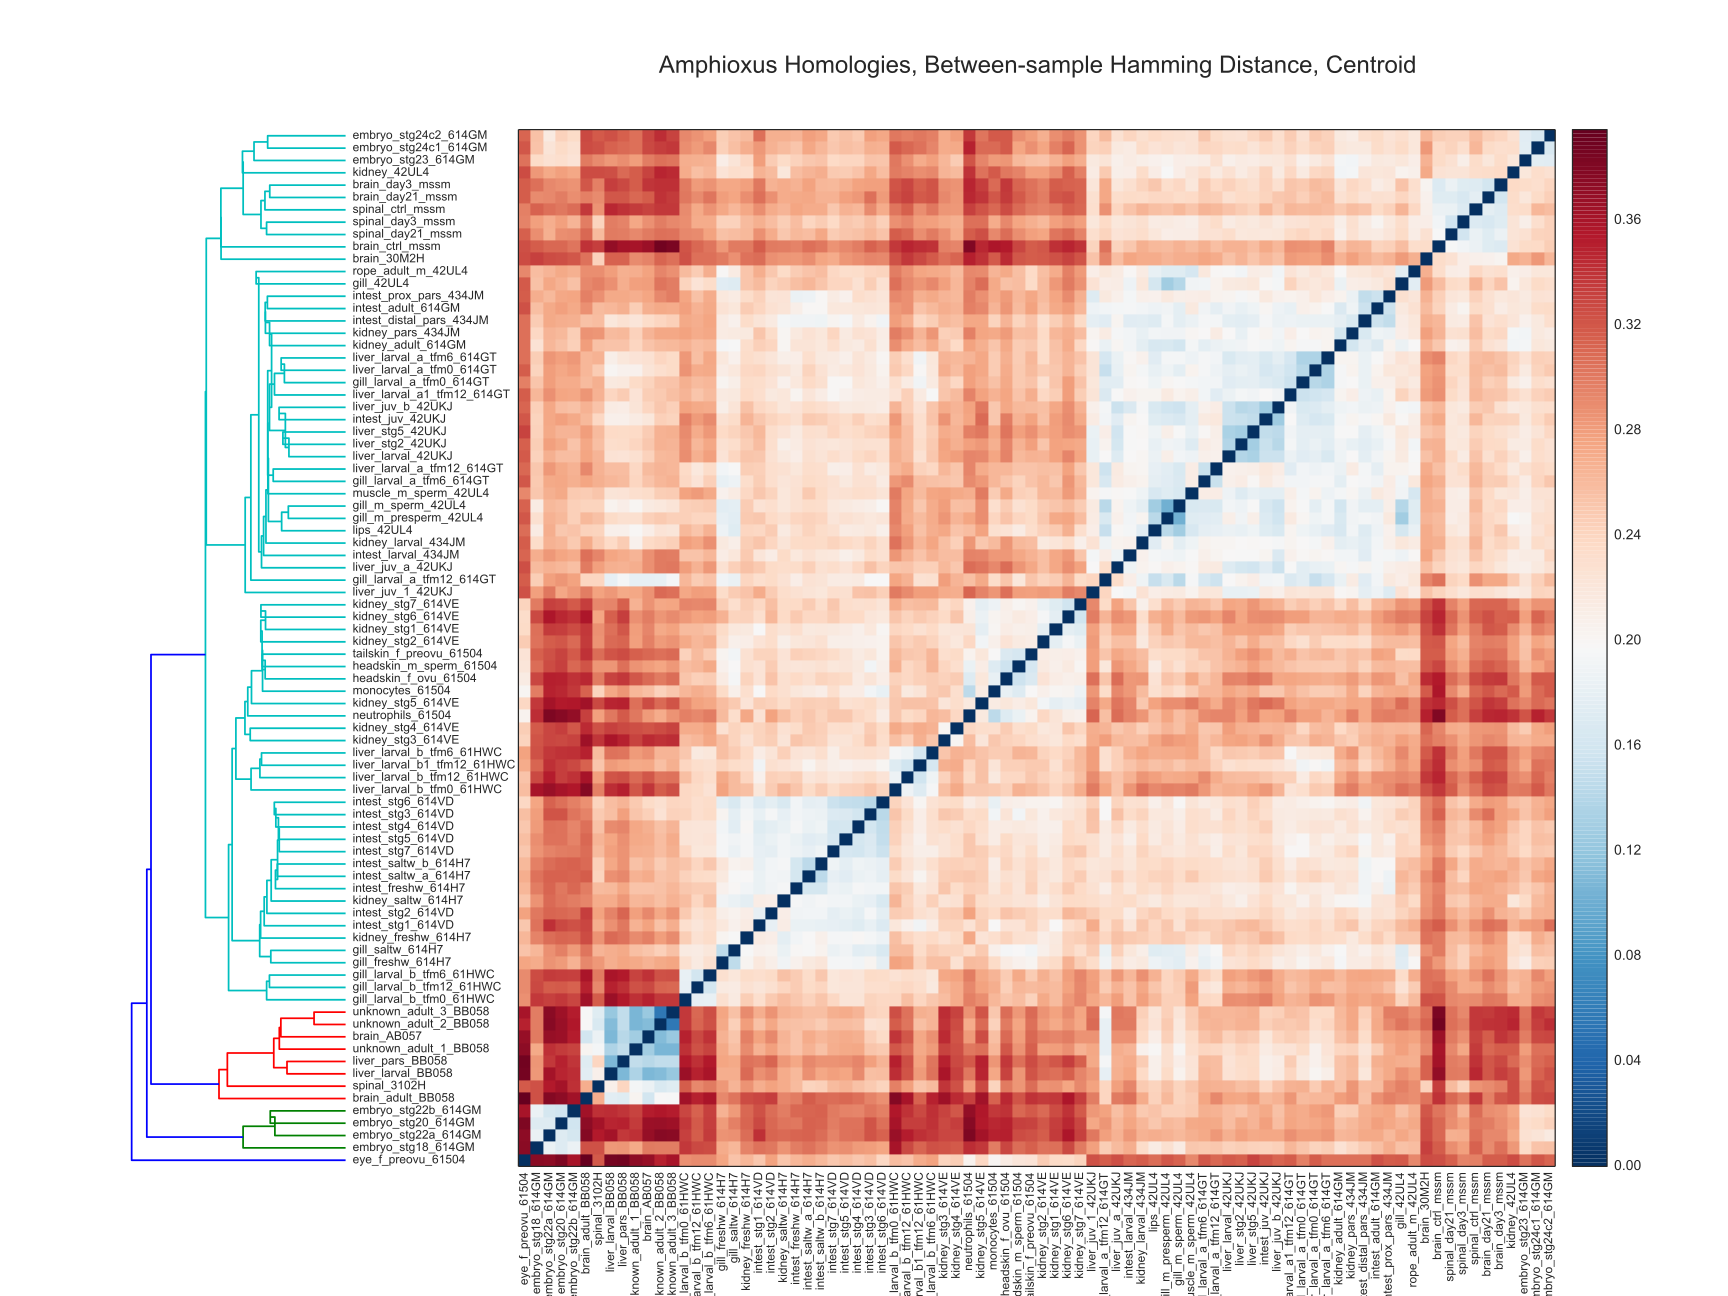
\includegraphics{amphioxus_dendro_hamming_centroid.svg}
\caption{amphioxus\_dendro\_hamming\_centroid}
\end{figure}

\begin{figure}[htbp]
\centering
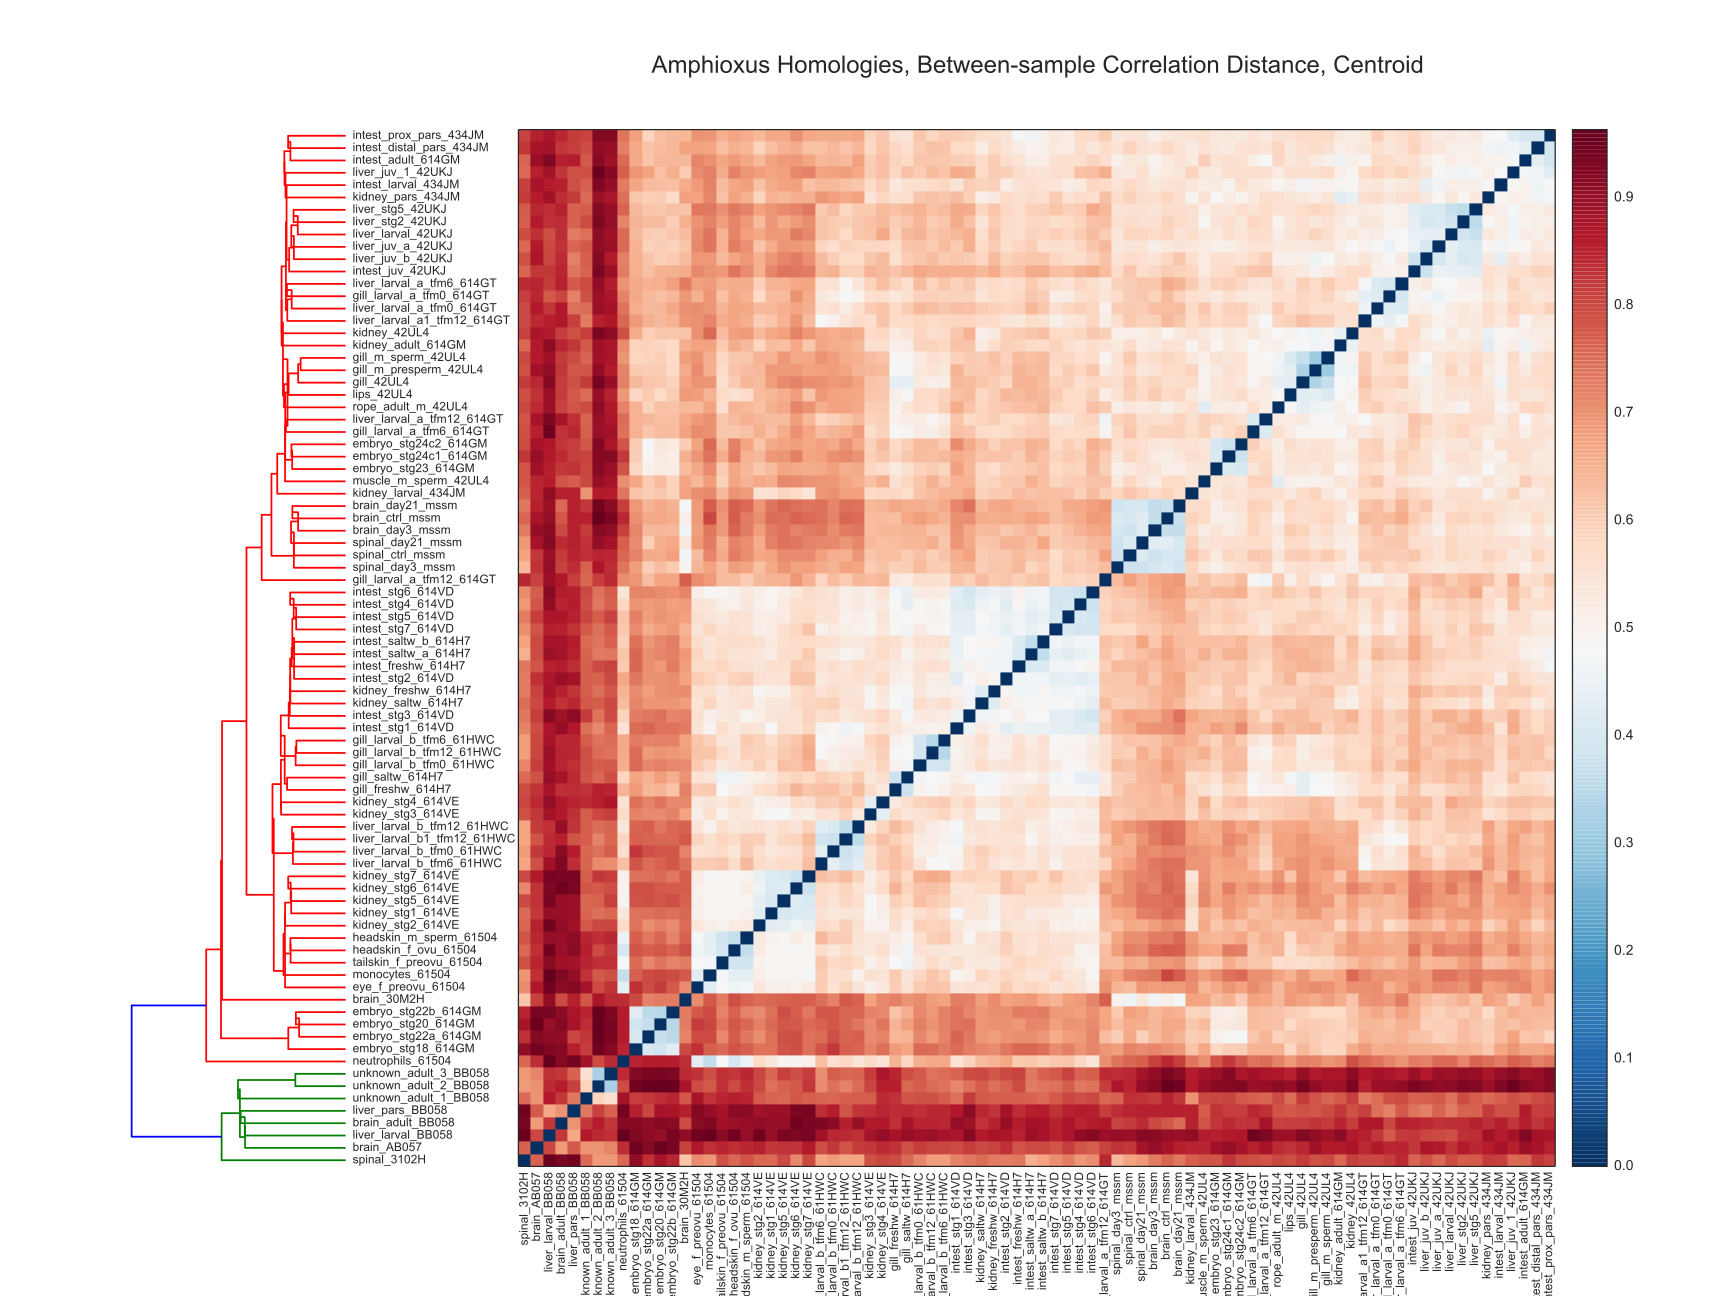
\includegraphics{amphioxus_dendro_correlation_centroid.svg}
\caption{amphioxus\_dendro\_correlation\_centroid}
\end{figure}

Next, we take transcripts homologous to mouse or zebrafish, but not to
amphioxus. Note that mouse and zebrafish and descendants of lamprey.

\begin{figure}[htbp]
\centering
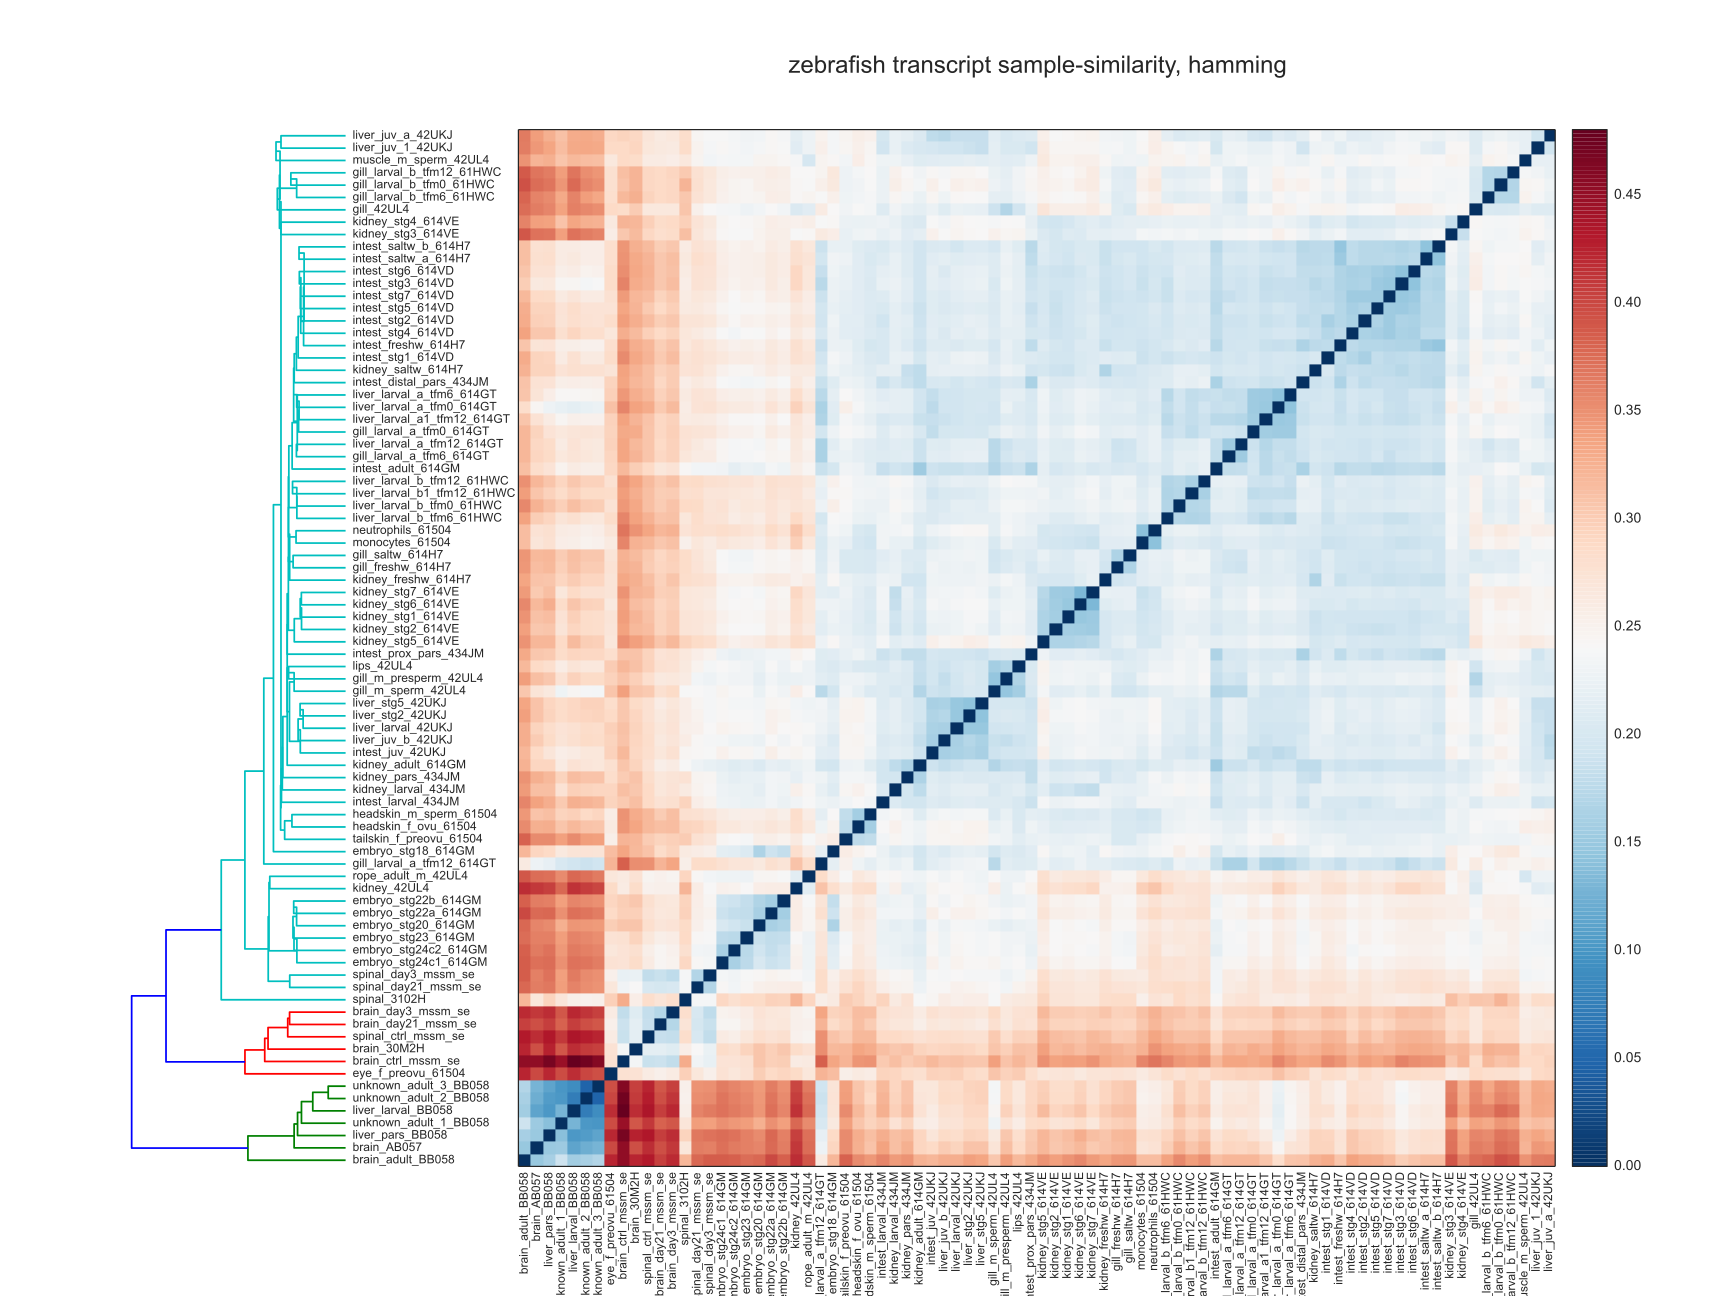
\includegraphics{zebrafish_dendro_hamming_centroid.svg}
\caption{zebrafish\_dendro\_hamming\_centroid}
\end{figure}

\begin{figure}[htbp]
\centering
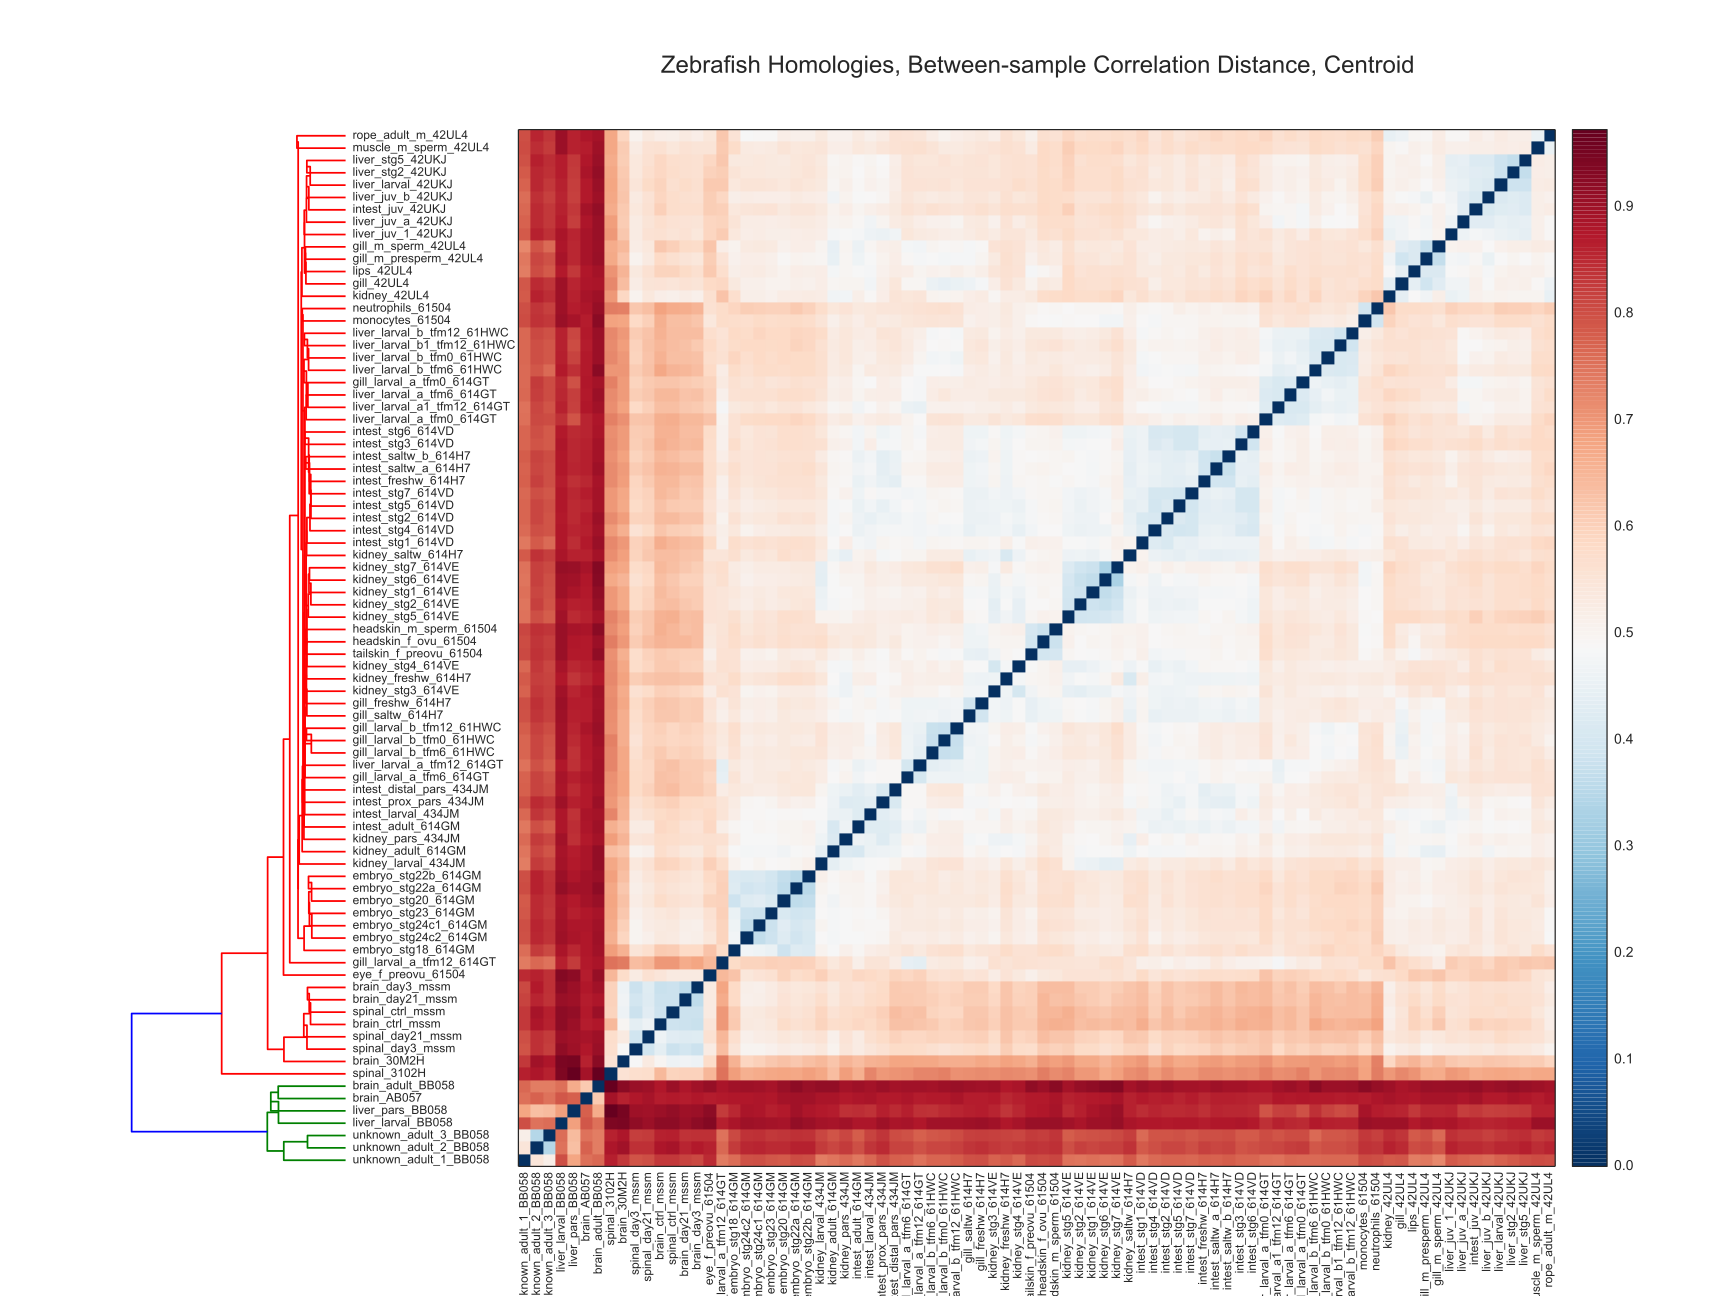
\includegraphics{zebrafish_dendro_correlation_centroid.svg}
\caption{zebrafish\_dendro\_correlation\_centroid}
\end{figure}


    \subsection{Conclusions}


    For now, I'm leaving out any of my interpretations of the data. I
welcome any and all feedback, thoughts, ideas -- especially any thoughts
on how this analysis (and other similar analyses) that I can perform are
useful for your research.


    % Add a bibliography block to the postdoc
    
    
    
    \end{document}
